\documentclass[14pt]{extarticle}
\usepackage[letterpaper, left=0.75in, right=0.75in, top=0.8in, bottom=0.8in,
  headheight=20pt, headsep=16pt, footskip=30pt]{geometry}
\usepackage{fontspec}
\setmainfont{texgyreheros}[Extension=.otf, UprightFont=*-regular,
  BoldFont=*-bold, ItalicFont=*-italic, BoldItalicFont=*-bolditalic]
\usepackage{tikz}
\usetikzlibrary{shapes.geometric, arrows.meta}
\usepackage{array}
\usepackage{fancyhdr}
\pagestyle{fancy}
\fancyhf{}
\fancyhead[L]{Week 8 / Rook race and Nim / K--1}
\fancyfoot[L]{Bellingham Math Circle / Week 8 / F08-K-v4}
\fancyfoot[R]{\thepage}
\renewcommand{\headrulewidth}{0pt}
\setlength{\parindent}{0pt}
\setlength{\parskip}{0pt}
\linespread{1.12}
\hyphenpenalty=10000
\exhyphenpenalty=10000
\newcommand{\prob}[1]{\textbf{Problem #1:}}
\begin{document}
\raggedright
\noindent\begin{minipage}[c]{4.85in}\raggedright
On your turn, slide the token straight left or straight down, toward the star's side, one or more squares. Whoever moves the token onto the star wins.
\end{minipage}\hfill\begin{minipage}[c]{1.8in}\raggedleft
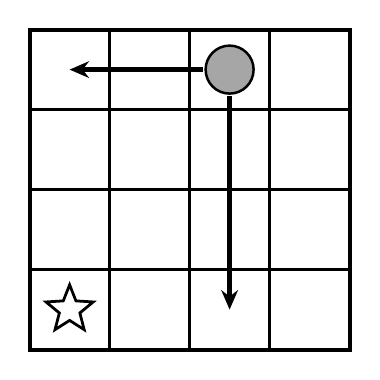
\begin{tikzpicture}[x=1in,y=1in]
\draw[line width=0.9pt] (0,0) grid[step=0.4] (1.6000,1.6000);
\draw[line width=1.4pt] (0,0) rectangle (1.6000,1.6000);
\node[star, star points=5, star point ratio=2.3, draw=black, line width=1.0pt, inner sep=0pt, outer sep=0pt, minimum size=0.248in] at (0.2000,0.2000) {};
\filldraw[fill=black!35, draw=black, line width=0.9pt] (1.0000,1.4000) circle (0.1200);
\draw[-{Stealth[length=7pt,width=6pt]}, line width=1.6pt] (0.8680,1.4000) -- (0.2000,1.4000);
\draw[-{Stealth[length=7pt,width=6pt]}, line width=1.6pt] (1.0000,1.2680) -- (1.0000,0.2000);
\end{tikzpicture}
\end{minipage}

\vspace{0.45in}
\prob{1} Play many games from the dot on each board. Circle if you would rather go first or second.

\vspace{0.35in}
\noindent \begin{minipage}[t]{3.3in}\centering
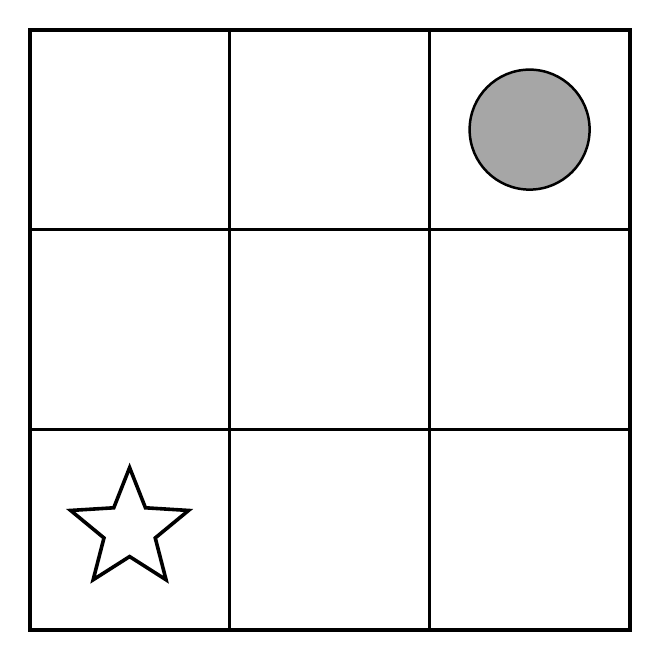
\begin{tikzpicture}[x=1in,y=1in]
\draw[line width=0.9pt] (0,0) grid[step=1.0] (3.0000,3.0000);
\draw[line width=1.4pt] (0,0) rectangle (3.0000,3.0000);
\node[star, star points=5, star point ratio=2.3, draw=black, line width=1.3pt, inner sep=0pt, outer sep=0pt, minimum size=0.620in] at (0.5000,0.5000) {};
\filldraw[fill=black!35, draw=black, line width=0.9pt] (2.5000,2.5000) circle (0.3000);
\end{tikzpicture}

\vspace{0.2in}
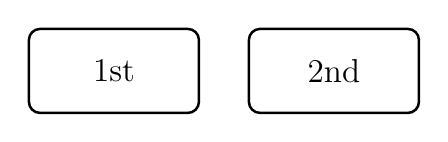
\begin{tikzpicture}[x=1in,y=1in]\draw[rounded corners=4pt, line width=0.9pt] (0,0) rectangle (0.85,0.42);\node at (0.425,0.21) {\large 1st};\draw[rounded corners=4pt, line width=0.9pt] (1.1,0) rectangle (1.9500000000000002,0.42);\node at (1.5250000000000001,0.21) {\large 2nd};\end{tikzpicture}
\end{minipage} \hfill \begin{minipage}[t]{3.3in}\centering
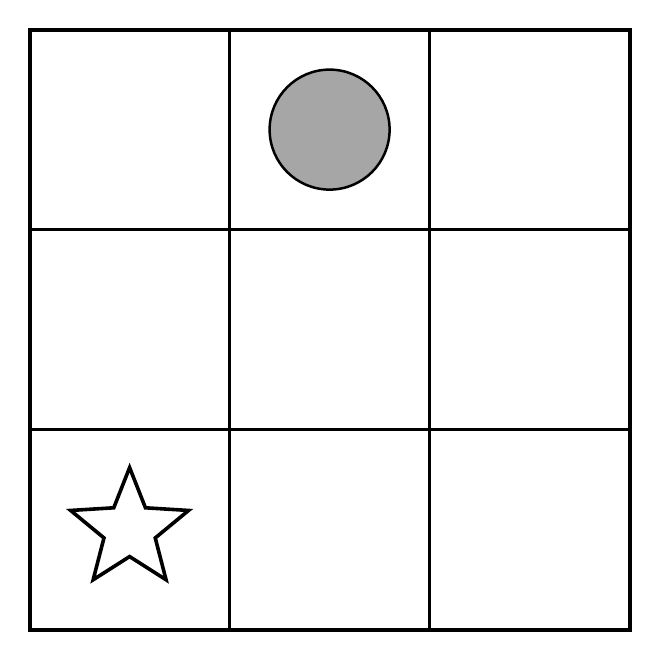
\begin{tikzpicture}[x=1in,y=1in]
\draw[line width=0.9pt] (0,0) grid[step=1.0] (3.0000,3.0000);
\draw[line width=1.4pt] (0,0) rectangle (3.0000,3.0000);
\node[star, star points=5, star point ratio=2.3, draw=black, line width=1.3pt, inner sep=0pt, outer sep=0pt, minimum size=0.620in] at (0.5000,0.5000) {};
\filldraw[fill=black!35, draw=black, line width=0.9pt] (1.5000,2.5000) circle (0.3000);
\end{tikzpicture}

\vspace{0.2in}
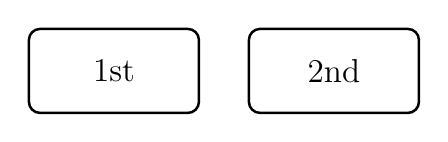
\begin{tikzpicture}[x=1in,y=1in]\draw[rounded corners=4pt, line width=0.9pt] (0,0) rectangle (0.85,0.42);\node at (0.425,0.21) {\large 1st};\draw[rounded corners=4pt, line width=0.9pt] (1.1,0) rectangle (1.9500000000000002,0.42);\node at (1.5250000000000001,0.21) {\large 2nd};\end{tikzpicture}
\end{minipage}
\newpage
\prob{2} Play many games from the dot on each board on this page and the next page. Circle if you would rather go first or second.

\vspace{0.1in}
\begin{center}
\begin{minipage}[c]{4.05in}
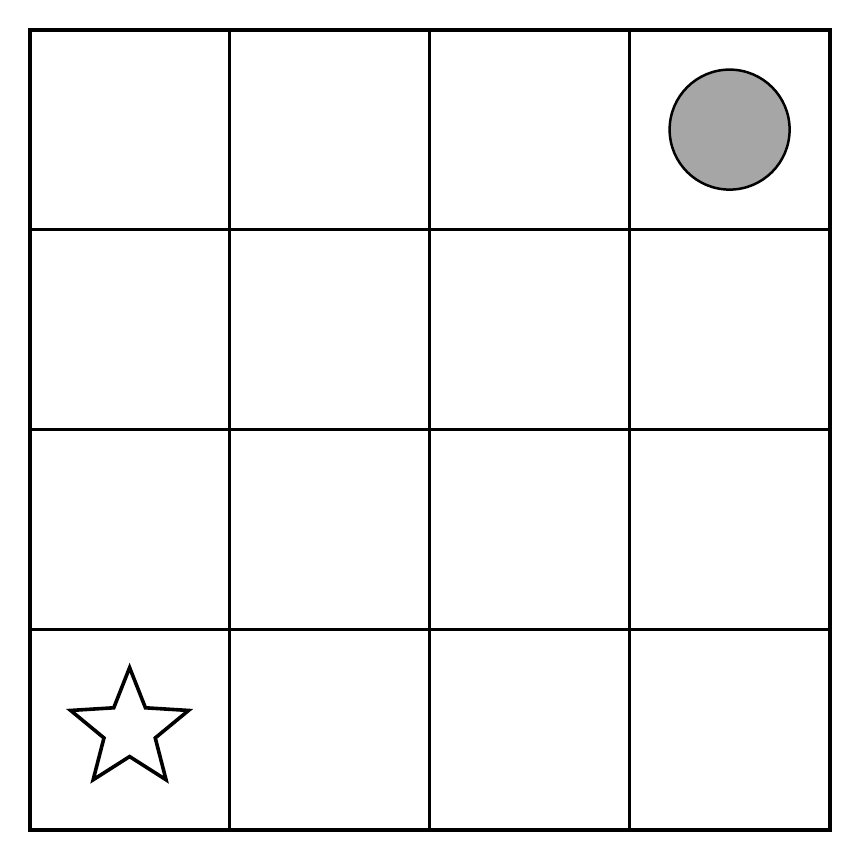
\begin{tikzpicture}[x=1in,y=1in]
\draw[line width=0.9pt] (0,0) grid[step=1.0] (4.0000,4.0000);
\draw[line width=1.4pt] (0,0) rectangle (4.0000,4.0000);
\node[star, star points=5, star point ratio=2.3, draw=black, line width=1.3pt, inner sep=0pt, outer sep=0pt, minimum size=0.620in] at (0.5000,0.5000) {};
\filldraw[fill=black!35, draw=black, line width=0.9pt] (3.5000,3.5000) circle (0.3000);
\end{tikzpicture}
\end{minipage}\hspace{0.45in}\begin{minipage}[c]{1.0in}
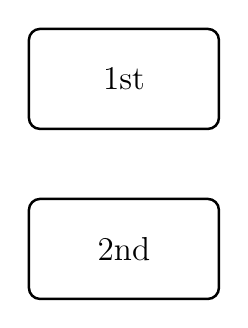
\begin{tikzpicture}[x=1in,y=1in]\draw[rounded corners=4pt, line width=0.9pt] (0,0) rectangle (0.95,0.5);\node at (0.475,0.25) {\large 1st};\draw[rounded corners=4pt, line width=0.9pt] (0,-0.85) rectangle (0.95,-0.35);\node at (0.475,-0.6) {\large 2nd};\end{tikzpicture}
\end{minipage}
\end{center}
\vspace{0.05in}
\begin{center}
\begin{minipage}[c]{4.05in}
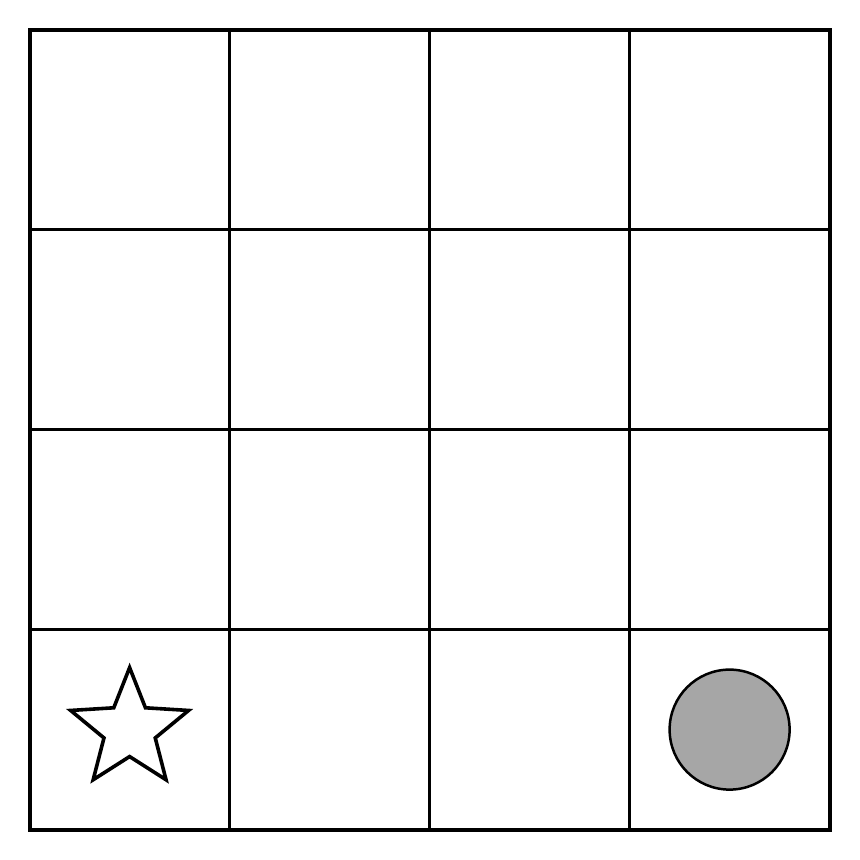
\begin{tikzpicture}[x=1in,y=1in]
\draw[line width=0.9pt] (0,0) grid[step=1.0] (4.0000,4.0000);
\draw[line width=1.4pt] (0,0) rectangle (4.0000,4.0000);
\node[star, star points=5, star point ratio=2.3, draw=black, line width=1.3pt, inner sep=0pt, outer sep=0pt, minimum size=0.620in] at (0.5000,0.5000) {};
\filldraw[fill=black!35, draw=black, line width=0.9pt] (3.5000,0.5000) circle (0.3000);
\end{tikzpicture}
\end{minipage}\hspace{0.45in}\begin{minipage}[c]{1.0in}
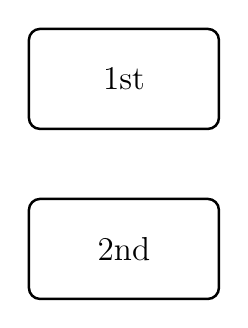
\begin{tikzpicture}[x=1in,y=1in]\draw[rounded corners=4pt, line width=0.9pt] (0,0) rectangle (0.95,0.5);\node at (0.475,0.25) {\large 1st};\draw[rounded corners=4pt, line width=0.9pt] (0,-0.85) rectangle (0.95,-0.35);\node at (0.475,-0.6) {\large 2nd};\end{tikzpicture}
\end{minipage}
\end{center}
\newpage
\vspace*{0.2in}
\begin{center}
\begin{minipage}[c]{4.05in}
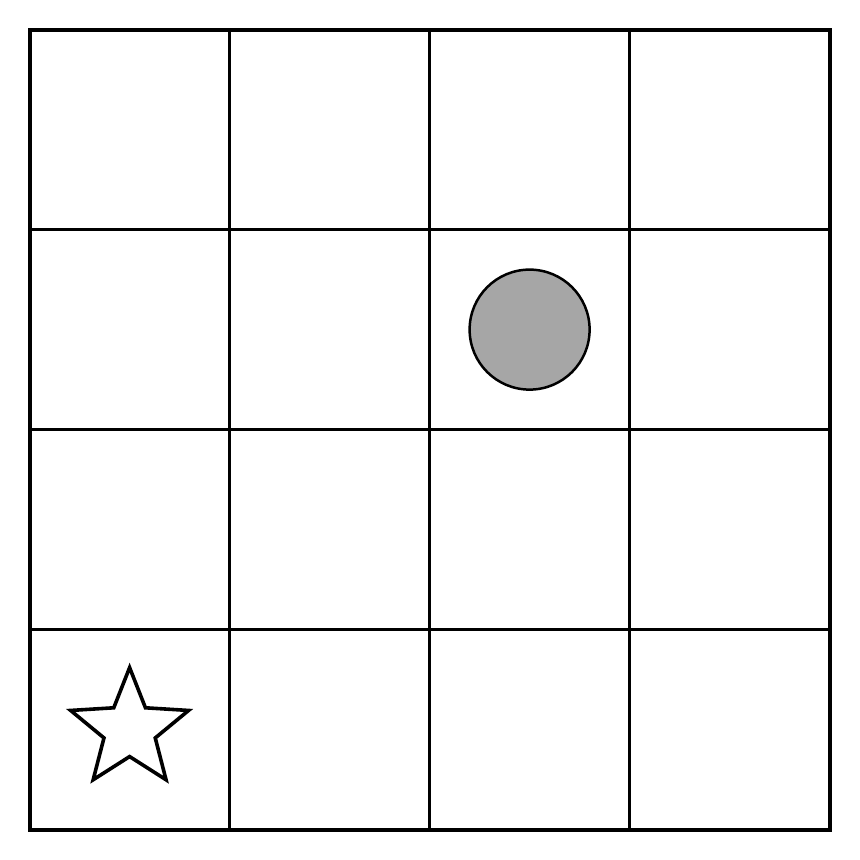
\begin{tikzpicture}[x=1in,y=1in]
\draw[line width=0.9pt] (0,0) grid[step=1.0] (4.0000,4.0000);
\draw[line width=1.4pt] (0,0) rectangle (4.0000,4.0000);
\node[star, star points=5, star point ratio=2.3, draw=black, line width=1.3pt, inner sep=0pt, outer sep=0pt, minimum size=0.620in] at (0.5000,0.5000) {};
\filldraw[fill=black!35, draw=black, line width=0.9pt] (2.5000,2.5000) circle (0.3000);
\end{tikzpicture}
\end{minipage}\hspace{0.45in}\begin{minipage}[c]{1.0in}
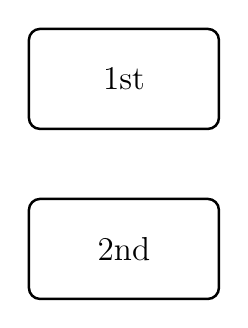
\begin{tikzpicture}[x=1in,y=1in]\draw[rounded corners=4pt, line width=0.9pt] (0,0) rectangle (0.95,0.5);\node at (0.475,0.25) {\large 1st};\draw[rounded corners=4pt, line width=0.9pt] (0,-0.85) rectangle (0.95,-0.35);\node at (0.475,-0.6) {\large 2nd};\end{tikzpicture}
\end{minipage}
\end{center}
\vspace{0.3in}
\begin{center}
\begin{minipage}[c]{4.05in}
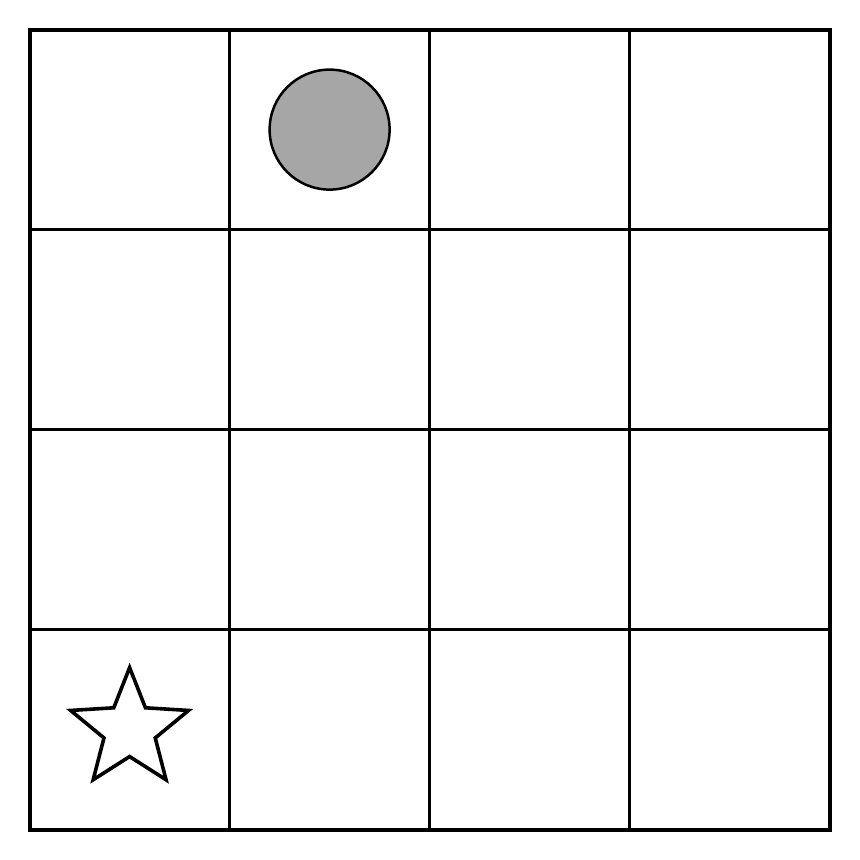
\begin{tikzpicture}[x=1in,y=1in]
\draw[line width=0.9pt] (0,0) grid[step=1.0] (4.0000,4.0000);
\draw[line width=1.4pt] (0,0) rectangle (4.0000,4.0000);
\node[star, star points=5, star point ratio=2.3, draw=black, line width=1.3pt, inner sep=0pt, outer sep=0pt, minimum size=0.620in] at (0.5000,0.5000) {};
\filldraw[fill=black!35, draw=black, line width=0.9pt] (1.5000,3.5000) circle (0.3000);
\end{tikzpicture}
\end{minipage}\hspace{0.45in}\begin{minipage}[c]{1.0in}
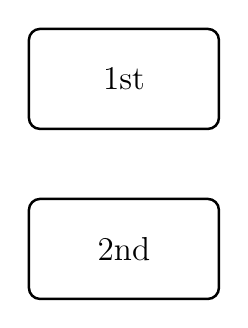
\begin{tikzpicture}[x=1in,y=1in]\draw[rounded corners=4pt, line width=0.9pt] (0,0) rectangle (0.95,0.5);\node at (0.475,0.25) {\large 1st};\draw[rounded corners=4pt, line width=0.9pt] (0,-0.85) rectangle (0.95,-0.35);\node at (0.475,-0.6) {\large 2nd};\end{tikzpicture}
\end{minipage}
\end{center}
\newpage
\prob{3} It is your turn, and the token is on the dot. Color the square you should move it to so that you can win.

\vspace{0.3in}
\noindent \begin{minipage}[t]{3.35in}\centering
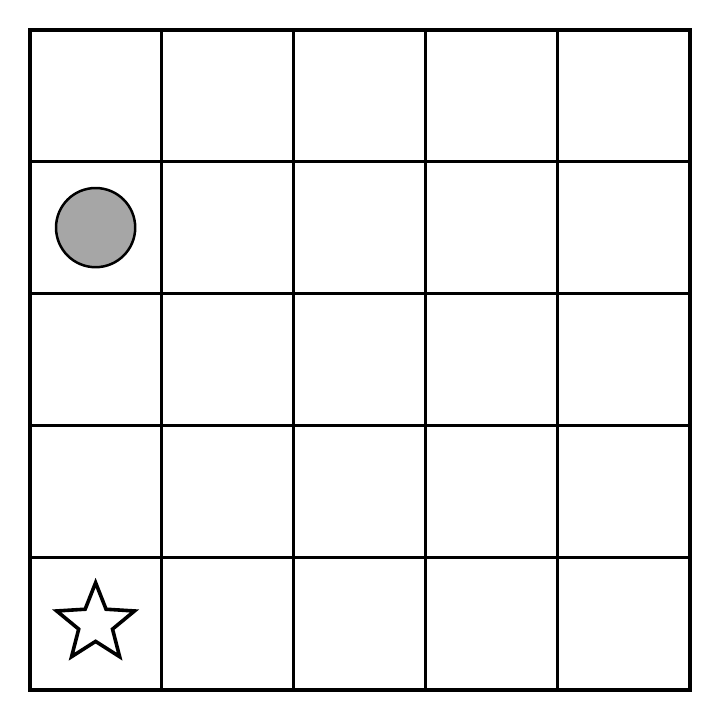
\begin{tikzpicture}[x=1in,y=1in]
\draw[line width=0.9pt] (0,0) grid[step=0.66] (3.3000,3.3000);
\draw[line width=1.4pt] (0,0) rectangle (3.3000,3.3000);
\node[star, star points=5, star point ratio=2.3, draw=black, line width=1.3pt, inner sep=0pt, outer sep=0pt, minimum size=0.409in] at (0.3300,0.3300) {};
\filldraw[fill=black!35, draw=black, line width=0.9pt] (0.3300,2.3100) circle (0.1980);
\end{tikzpicture}
\end{minipage} \hfill \begin{minipage}[t]{3.35in}\centering
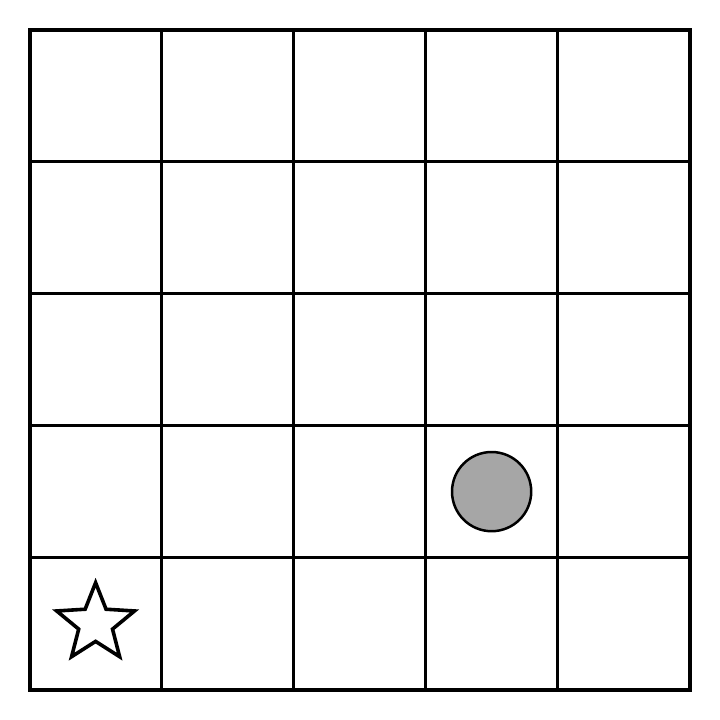
\begin{tikzpicture}[x=1in,y=1in]
\draw[line width=0.9pt] (0,0) grid[step=0.66] (3.3000,3.3000);
\draw[line width=1.4pt] (0,0) rectangle (3.3000,3.3000);
\node[star, star points=5, star point ratio=2.3, draw=black, line width=1.3pt, inner sep=0pt, outer sep=0pt, minimum size=0.409in] at (0.3300,0.3300) {};
\filldraw[fill=black!35, draw=black, line width=0.9pt] (2.3100,0.9900) circle (0.1980);
\end{tikzpicture}
\end{minipage}

\vspace{0.45in}

\noindent \begin{minipage}[t]{3.35in}\centering
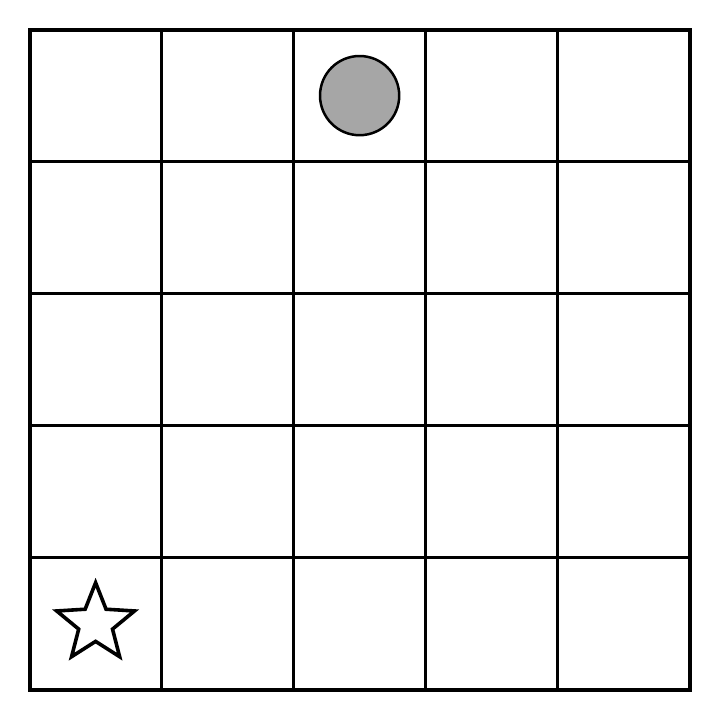
\begin{tikzpicture}[x=1in,y=1in]
\draw[line width=0.9pt] (0,0) grid[step=0.66] (3.3000,3.3000);
\draw[line width=1.4pt] (0,0) rectangle (3.3000,3.3000);
\node[star, star points=5, star point ratio=2.3, draw=black, line width=1.3pt, inner sep=0pt, outer sep=0pt, minimum size=0.409in] at (0.3300,0.3300) {};
\filldraw[fill=black!35, draw=black, line width=0.9pt] (1.6500,2.9700) circle (0.1980);
\end{tikzpicture}
\end{minipage} \hfill \begin{minipage}[t]{3.35in}\centering
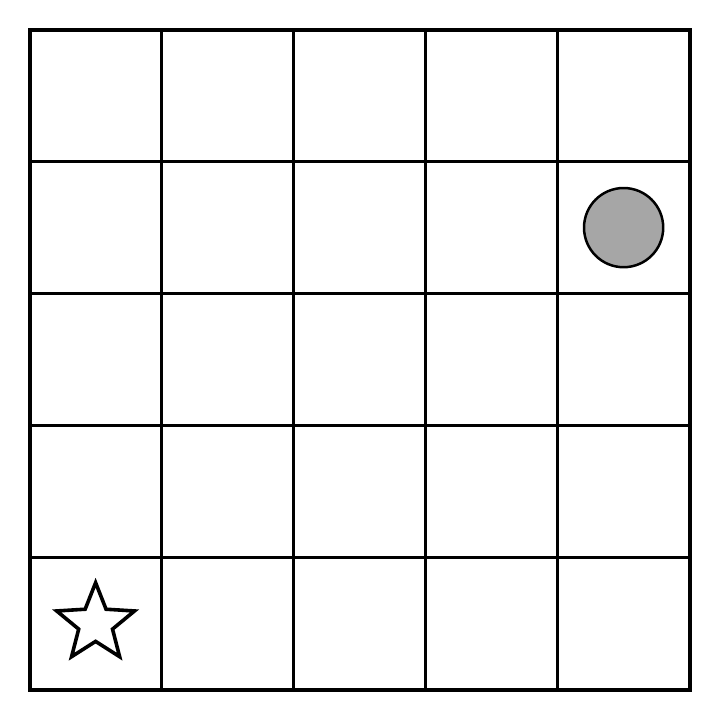
\begin{tikzpicture}[x=1in,y=1in]
\draw[line width=0.9pt] (0,0) grid[step=0.66] (3.3000,3.3000);
\draw[line width=1.4pt] (0,0) rectangle (3.3000,3.3000);
\node[star, star points=5, star point ratio=2.3, draw=black, line width=1.3pt, inner sep=0pt, outer sep=0pt, minimum size=0.409in] at (0.3300,0.3300) {};
\filldraw[fill=black!35, draw=black, line width=0.9pt] (2.9700,2.3100) circle (0.1980);
\end{tikzpicture}
\end{minipage}
\newpage
\prob{4} Play many games on this board, starting on any square except the star. Color every square you want to move the token to.

\vspace{0.3in}
\begin{center}
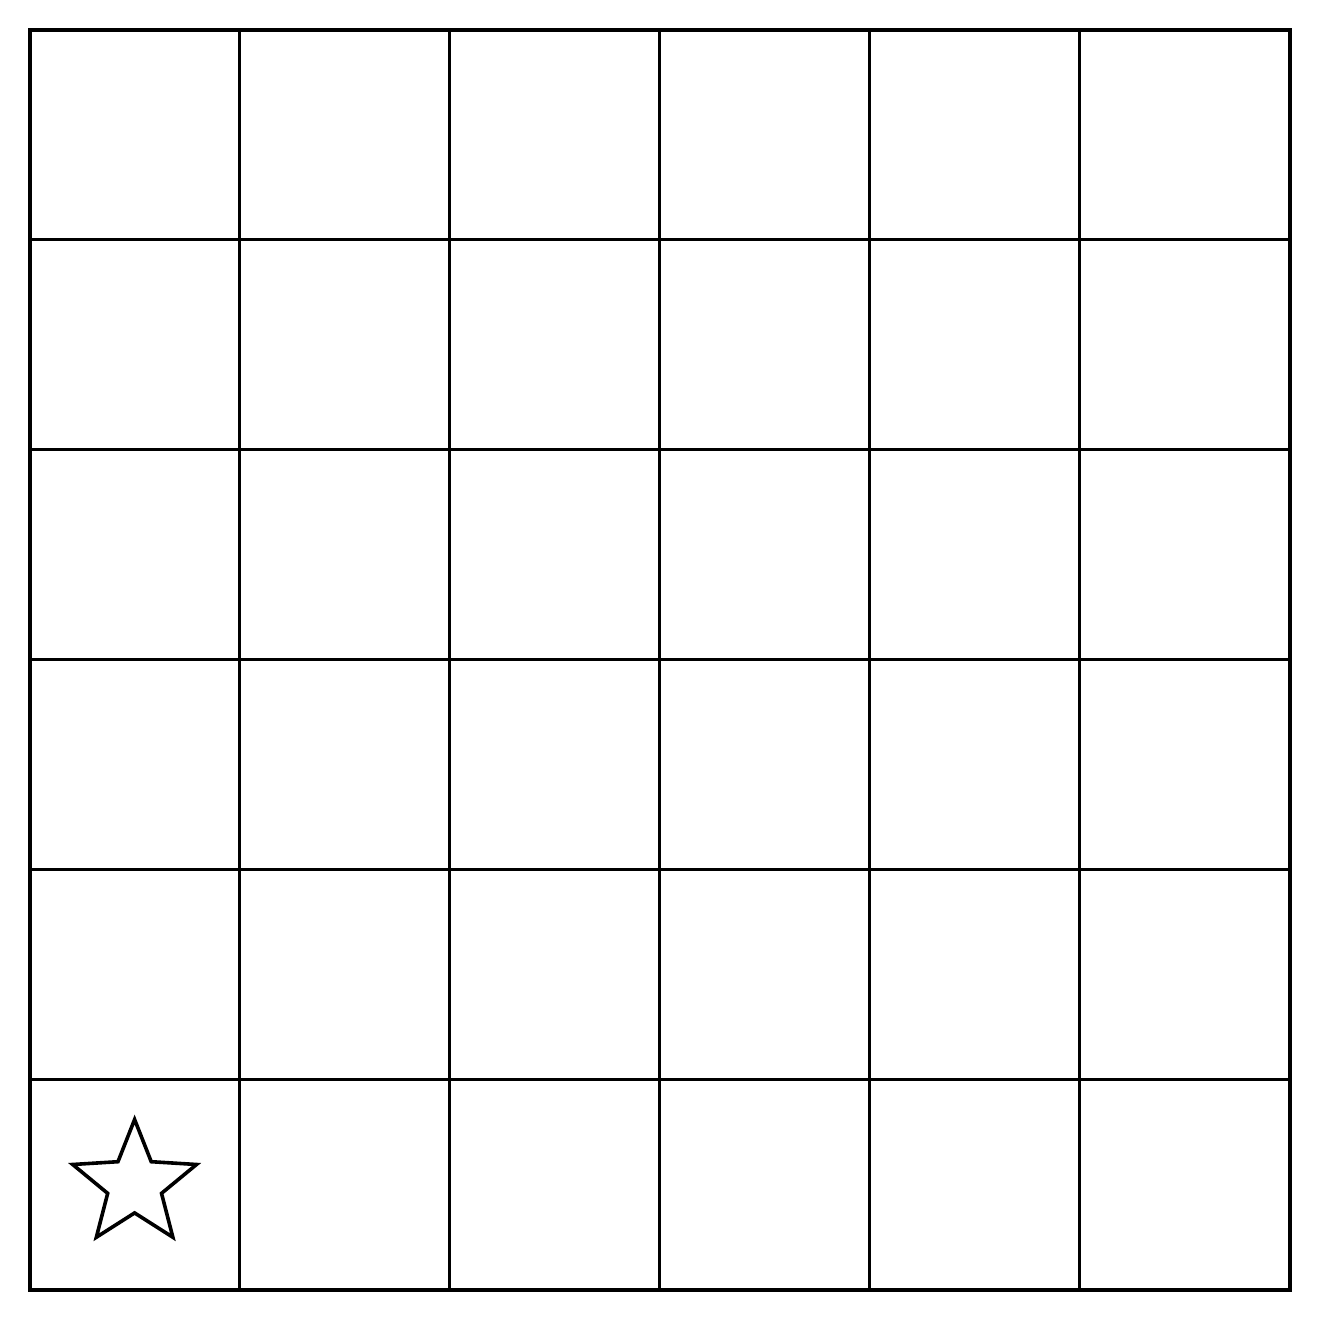
\begin{tikzpicture}[x=1in,y=1in]
\draw[line width=0.9pt] (0,0) grid[step=1.05] (6.3000,6.3000);
\draw[line width=1.4pt] (0,0) rectangle (6.3000,6.3000);
\node[star, star points=5, star point ratio=2.3, draw=black, line width=1.3pt, inner sep=0pt, outer sep=0pt, minimum size=0.651in] at (0.5250,0.5250) {};
\end{tikzpicture}
\end{center}
\newpage
\prob{5} On your turn, take one or more counters from one pile, and whoever takes the last counter wins. Play with each pair of piles and circle if you would rather go first or second.

\vspace{0.3in}
\noindent \begin{minipage}[t]{3.35in}\centering
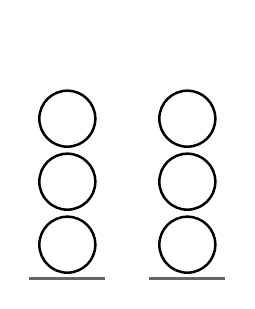
\begin{tikzpicture}[x=1in,y=1in]
\path (0,-0.03) -- (0,1.2250);
\draw[line width=0.9pt, fill=white] (0.0000,0.1400) circle (0.1400);
\draw[line width=0.9pt, fill=white] (0.0000,0.4550) circle (0.1400);
\draw[line width=0.9pt, fill=white] (0.0000,0.7700) circle (0.1400);
\draw[line width=1.2pt, black!60] (-0.1900,-0.03) -- (0.1900,-0.03);
\draw[line width=0.9pt, fill=white] (0.6000,0.1400) circle (0.1400);
\draw[line width=0.9pt, fill=white] (0.6000,0.4550) circle (0.1400);
\draw[line width=0.9pt, fill=white] (0.6000,0.7700) circle (0.1400);
\draw[line width=1.2pt, black!60] (0.4100,-0.03) -- (0.7900,-0.03);
\end{tikzpicture}

\vspace{0.15in}
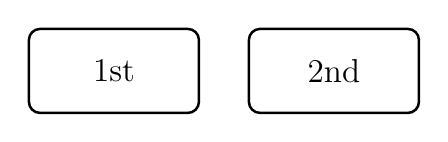
\begin{tikzpicture}[x=1in,y=1in]\draw[rounded corners=4pt, line width=0.9pt] (0,0) rectangle (0.85,0.42);\node at (0.425,0.21) {\large 1st};\draw[rounded corners=4pt, line width=0.9pt] (1.1,0) rectangle (1.9500000000000002,0.42);\node at (1.5250000000000001,0.21) {\large 2nd};\end{tikzpicture}
\end{minipage} \hfill \begin{minipage}[t]{3.35in}\centering
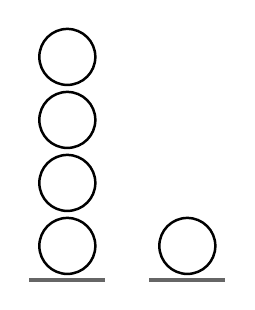
\begin{tikzpicture}[x=1in,y=1in]
\path (0,-0.03) -- (0,1.2250);
\draw[line width=0.9pt, fill=white] (0.0000,0.1400) circle (0.1400);
\draw[line width=0.9pt, fill=white] (0.0000,0.4550) circle (0.1400);
\draw[line width=0.9pt, fill=white] (0.0000,0.7700) circle (0.1400);
\draw[line width=0.9pt, fill=white] (0.0000,1.0850) circle (0.1400);
\draw[line width=1.2pt, black!60] (-0.1900,-0.03) -- (0.1900,-0.03);
\draw[line width=0.9pt, fill=white] (0.6000,0.1400) circle (0.1400);
\draw[line width=1.2pt, black!60] (0.4100,-0.03) -- (0.7900,-0.03);
\end{tikzpicture}

\vspace{0.15in}
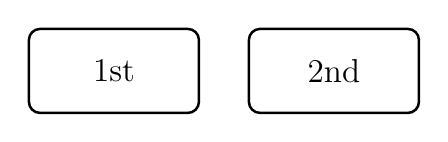
\begin{tikzpicture}[x=1in,y=1in]\draw[rounded corners=4pt, line width=0.9pt] (0,0) rectangle (0.85,0.42);\node at (0.425,0.21) {\large 1st};\draw[rounded corners=4pt, line width=0.9pt] (1.1,0) rectangle (1.9500000000000002,0.42);\node at (1.5250000000000001,0.21) {\large 2nd};\end{tikzpicture}
\end{minipage}

\vspace{0.4in}

\noindent \begin{minipage}[t]{3.35in}\centering
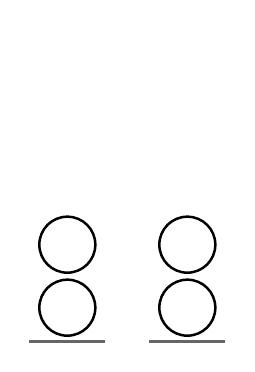
\begin{tikzpicture}[x=1in,y=1in]
\path (0,-0.03) -- (0,1.5400);
\draw[line width=0.9pt, fill=white] (0.0000,0.1400) circle (0.1400);
\draw[line width=0.9pt, fill=white] (0.0000,0.4550) circle (0.1400);
\draw[line width=1.2pt, black!60] (-0.1900,-0.03) -- (0.1900,-0.03);
\draw[line width=0.9pt, fill=white] (0.6000,0.1400) circle (0.1400);
\draw[line width=0.9pt, fill=white] (0.6000,0.4550) circle (0.1400);
\draw[line width=1.2pt, black!60] (0.4100,-0.03) -- (0.7900,-0.03);
\end{tikzpicture}

\vspace{0.15in}
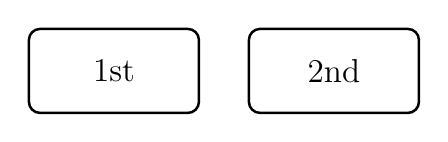
\begin{tikzpicture}[x=1in,y=1in]\draw[rounded corners=4pt, line width=0.9pt] (0,0) rectangle (0.85,0.42);\node at (0.425,0.21) {\large 1st};\draw[rounded corners=4pt, line width=0.9pt] (1.1,0) rectangle (1.9500000000000002,0.42);\node at (1.5250000000000001,0.21) {\large 2nd};\end{tikzpicture}
\end{minipage} \hfill \begin{minipage}[t]{3.35in}\centering
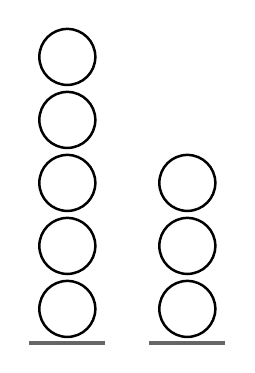
\begin{tikzpicture}[x=1in,y=1in]
\path (0,-0.03) -- (0,1.5400);
\draw[line width=0.9pt, fill=white] (0.0000,0.1400) circle (0.1400);
\draw[line width=0.9pt, fill=white] (0.0000,0.4550) circle (0.1400);
\draw[line width=0.9pt, fill=white] (0.0000,0.7700) circle (0.1400);
\draw[line width=0.9pt, fill=white] (0.0000,1.0850) circle (0.1400);
\draw[line width=0.9pt, fill=white] (0.0000,1.4000) circle (0.1400);
\draw[line width=1.2pt, black!60] (-0.1900,-0.03) -- (0.1900,-0.03);
\draw[line width=0.9pt, fill=white] (0.6000,0.1400) circle (0.1400);
\draw[line width=0.9pt, fill=white] (0.6000,0.4550) circle (0.1400);
\draw[line width=0.9pt, fill=white] (0.6000,0.7700) circle (0.1400);
\draw[line width=1.2pt, black!60] (0.4100,-0.03) -- (0.7900,-0.03);
\end{tikzpicture}

\vspace{0.15in}
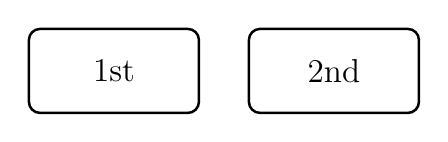
\begin{tikzpicture}[x=1in,y=1in]\draw[rounded corners=4pt, line width=0.9pt] (0,0) rectangle (0.85,0.42);\node at (0.425,0.21) {\large 1st};\draw[rounded corners=4pt, line width=0.9pt] (1.1,0) rectangle (1.9500000000000002,0.42);\node at (1.5250000000000001,0.21) {\large 2nd};\end{tikzpicture}
\end{minipage}
\vspace{0.5in}

\prob{6} Your partner goes first with these two piles of 7. Show the adult how you can always win.

\vspace{0.2in}
\begin{center}
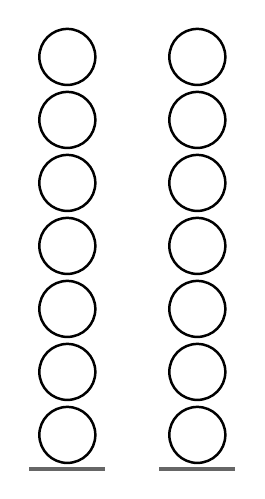
\begin{tikzpicture}[x=1in,y=1in]
\draw[line width=0.9pt, fill=white] (0.0000,0.1400) circle (0.1400);
\draw[line width=0.9pt, fill=white] (0.0000,0.4550) circle (0.1400);
\draw[line width=0.9pt, fill=white] (0.0000,0.7700) circle (0.1400);
\draw[line width=0.9pt, fill=white] (0.0000,1.0850) circle (0.1400);
\draw[line width=0.9pt, fill=white] (0.0000,1.4000) circle (0.1400);
\draw[line width=0.9pt, fill=white] (0.0000,1.7150) circle (0.1400);
\draw[line width=0.9pt, fill=white] (0.0000,2.0300) circle (0.1400);
\draw[line width=1.2pt, black!60] (-0.1900,-0.03) -- (0.1900,-0.03);
\draw[line width=0.9pt, fill=white] (0.6500,0.1400) circle (0.1400);
\draw[line width=0.9pt, fill=white] (0.6500,0.4550) circle (0.1400);
\draw[line width=0.9pt, fill=white] (0.6500,0.7700) circle (0.1400);
\draw[line width=0.9pt, fill=white] (0.6500,1.0850) circle (0.1400);
\draw[line width=0.9pt, fill=white] (0.6500,1.4000) circle (0.1400);
\draw[line width=0.9pt, fill=white] (0.6500,1.7150) circle (0.1400);
\draw[line width=0.9pt, fill=white] (0.6500,2.0300) circle (0.1400);
\draw[line width=1.2pt, black!60] (0.4600,-0.03) -- (0.8400,-0.03);
\end{tikzpicture}
\end{center}
\newpage
\prob{7} Your partner goes first, with the token in the corner farthest from the star on the separate 8-by-8 board. Show the adult how you can always win.

\vspace{0.15in}
\begin{center}
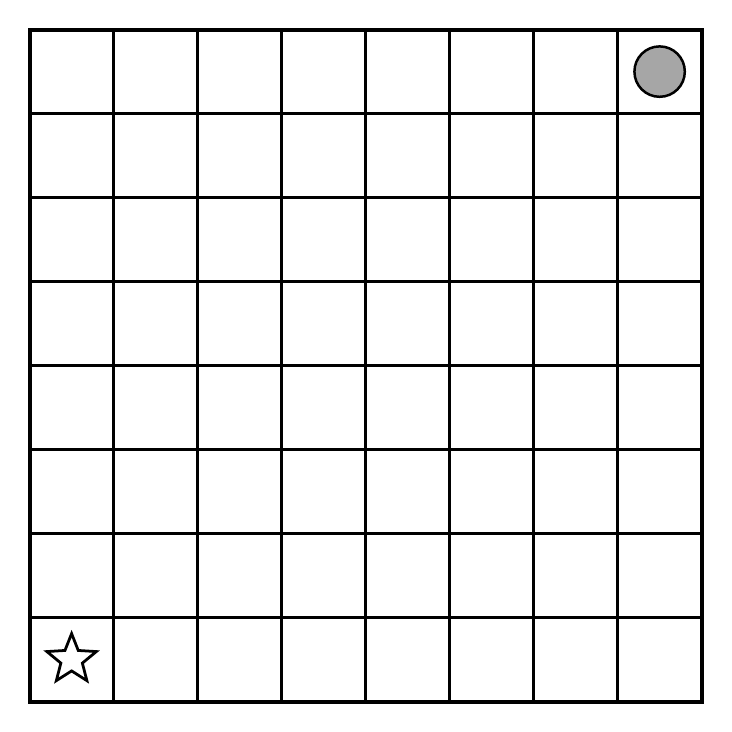
\begin{tikzpicture}[x=1in,y=1in]
\draw[line width=0.9pt] (0,0) grid[step=0.42] (3.3600,3.3600);
\draw[line width=1.4pt] (0,0) rectangle (3.3600,3.3600);
\node[star, star points=5, star point ratio=2.3, draw=black, line width=1.0pt, inner sep=0pt, outer sep=0pt, minimum size=0.260in] at (0.2100,0.2100) {};
\filldraw[fill=black!35, draw=black, line width=0.9pt] (3.1500,3.1500) circle (0.1260);
\end{tikzpicture}
\end{center}
\vspace{0.3in}

\prob{8} Make each set of three piles with counters and play many games. Circle if you would rather go first or second.

\vspace{0.25in}
\noindent \begin{minipage}[t]{3.35in}\centering
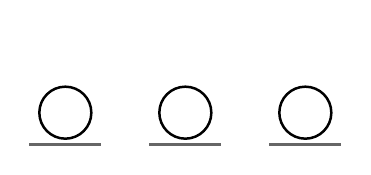
\begin{tikzpicture}[x=1in,y=1in]
\path (0,-0.03) -- (0,0.5550);
\draw[line width=0.9pt, fill=white] (0.0000,0.1300) circle (0.1300);
\draw[line width=1.2pt, black!60] (-0.1800,-0.03) -- (0.1800,-0.03);
\draw[line width=0.9pt, fill=white] (0.6000,0.1300) circle (0.1300);
\draw[line width=1.2pt, black!60] (0.4200,-0.03) -- (0.7800,-0.03);
\draw[line width=0.9pt, fill=white] (1.2000,0.1300) circle (0.1300);
\draw[line width=1.2pt, black!60] (1.0200,-0.03) -- (1.3800,-0.03);
\end{tikzpicture}

\vspace{0.12in}
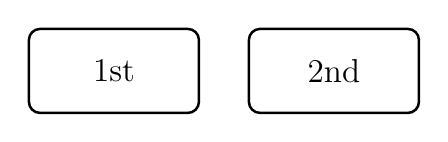
\begin{tikzpicture}[x=1in,y=1in]\draw[rounded corners=4pt, line width=0.9pt] (0,0) rectangle (0.85,0.42);\node at (0.425,0.21) {\large 1st};\draw[rounded corners=4pt, line width=0.9pt] (1.1,0) rectangle (1.9500000000000002,0.42);\node at (1.5250000000000001,0.21) {\large 2nd};\end{tikzpicture}
\end{minipage} \hfill \begin{minipage}[t]{3.35in}\centering
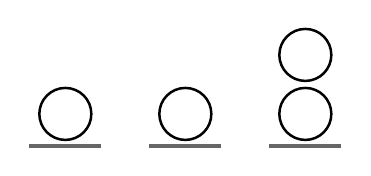
\begin{tikzpicture}[x=1in,y=1in]
\path (0,-0.03) -- (0,0.5550);
\draw[line width=0.9pt, fill=white] (0.0000,0.1300) circle (0.1300);
\draw[line width=1.2pt, black!60] (-0.1800,-0.03) -- (0.1800,-0.03);
\draw[line width=0.9pt, fill=white] (0.6000,0.1300) circle (0.1300);
\draw[line width=1.2pt, black!60] (0.4200,-0.03) -- (0.7800,-0.03);
\draw[line width=0.9pt, fill=white] (1.2000,0.1300) circle (0.1300);
\draw[line width=0.9pt, fill=white] (1.2000,0.4250) circle (0.1300);
\draw[line width=1.2pt, black!60] (1.0200,-0.03) -- (1.3800,-0.03);
\end{tikzpicture}

\vspace{0.12in}
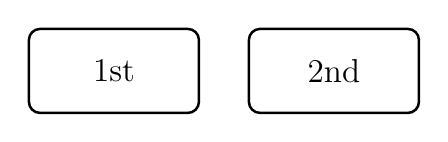
\begin{tikzpicture}[x=1in,y=1in]\draw[rounded corners=4pt, line width=0.9pt] (0,0) rectangle (0.85,0.42);\node at (0.425,0.21) {\large 1st};\draw[rounded corners=4pt, line width=0.9pt] (1.1,0) rectangle (1.9500000000000002,0.42);\node at (1.5250000000000001,0.21) {\large 2nd};\end{tikzpicture}
\end{minipage}

\vspace{0.3in}

\noindent \begin{minipage}[t]{3.35in}\centering
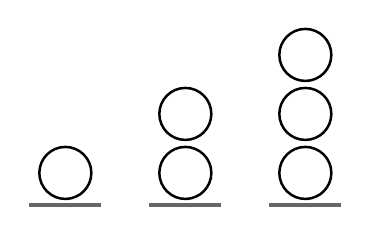
\begin{tikzpicture}[x=1in,y=1in]
\path (0,-0.03) -- (0,0.8500);
\draw[line width=0.9pt, fill=white] (0.0000,0.1300) circle (0.1300);
\draw[line width=1.2pt, black!60] (-0.1800,-0.03) -- (0.1800,-0.03);
\draw[line width=0.9pt, fill=white] (0.6000,0.1300) circle (0.1300);
\draw[line width=0.9pt, fill=white] (0.6000,0.4250) circle (0.1300);
\draw[line width=1.2pt, black!60] (0.4200,-0.03) -- (0.7800,-0.03);
\draw[line width=0.9pt, fill=white] (1.2000,0.1300) circle (0.1300);
\draw[line width=0.9pt, fill=white] (1.2000,0.4250) circle (0.1300);
\draw[line width=0.9pt, fill=white] (1.2000,0.7200) circle (0.1300);
\draw[line width=1.2pt, black!60] (1.0200,-0.03) -- (1.3800,-0.03);
\end{tikzpicture}

\vspace{0.12in}
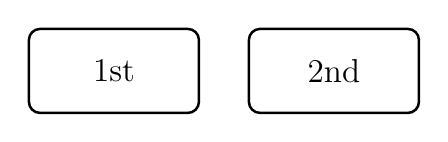
\begin{tikzpicture}[x=1in,y=1in]\draw[rounded corners=4pt, line width=0.9pt] (0,0) rectangle (0.85,0.42);\node at (0.425,0.21) {\large 1st};\draw[rounded corners=4pt, line width=0.9pt] (1.1,0) rectangle (1.9500000000000002,0.42);\node at (1.5250000000000001,0.21) {\large 2nd};\end{tikzpicture}
\end{minipage} \hfill \begin{minipage}[t]{3.35in}\centering
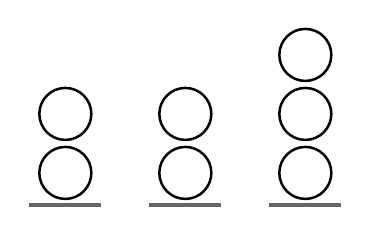
\begin{tikzpicture}[x=1in,y=1in]
\path (0,-0.03) -- (0,0.8500);
\draw[line width=0.9pt, fill=white] (0.0000,0.1300) circle (0.1300);
\draw[line width=0.9pt, fill=white] (0.0000,0.4250) circle (0.1300);
\draw[line width=1.2pt, black!60] (-0.1800,-0.03) -- (0.1800,-0.03);
\draw[line width=0.9pt, fill=white] (0.6000,0.1300) circle (0.1300);
\draw[line width=0.9pt, fill=white] (0.6000,0.4250) circle (0.1300);
\draw[line width=1.2pt, black!60] (0.4200,-0.03) -- (0.7800,-0.03);
\draw[line width=0.9pt, fill=white] (1.2000,0.1300) circle (0.1300);
\draw[line width=0.9pt, fill=white] (1.2000,0.4250) circle (0.1300);
\draw[line width=0.9pt, fill=white] (1.2000,0.7200) circle (0.1300);
\draw[line width=1.2pt, black!60] (1.0200,-0.03) -- (1.3800,-0.03);
\end{tikzpicture}

\vspace{0.12in}
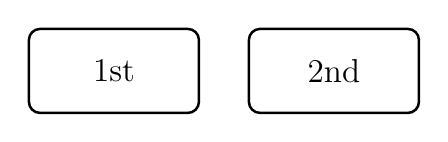
\begin{tikzpicture}[x=1in,y=1in]\draw[rounded corners=4pt, line width=0.9pt] (0,0) rectangle (0.85,0.42);\node at (0.425,0.21) {\large 1st};\draw[rounded corners=4pt, line width=0.9pt] (1.1,0) rectangle (1.9500000000000002,0.42);\node at (1.5250000000000001,0.21) {\large 2nd};\end{tikzpicture}
\end{minipage}

\end{document}
